\documentclass[14pt]{extbook}
\usepackage{multicol, enumerate, enumitem, hyperref, color, soul, setspace, parskip, fancyhdr} %General Packages
\usepackage{amssymb, amsthm, amsmath, bbm, latexsym, units, mathtools} %Math Packages
\everymath{\displaystyle} %All math in Display Style
% Packages with additional options
\usepackage[headsep=0.5cm,headheight=12pt, left=1 in,right= 1 in,top= 1 in,bottom= 1 in]{geometry}
\usepackage[usenames,dvipsnames]{xcolor}
\usepackage{dashrule}  % Package to use the command below to create lines between items
\newcommand{\litem}[1]{\item#1\hspace*{-1cm}\rule{\textwidth}{0.4pt}}
\pagestyle{fancy}
\lhead{Makeup Progress Quiz 3}
\chead{}
\rhead{Version C}
\lfoot{4315-3397}
\cfoot{}
\rfoot{Fall 2020}
\begin{document}

\begin{enumerate}
\litem{
Write the equation of the graph presented below in the form $f(x)=ax^2+bx+c$, assuming  $a=1$ or $a=-1$. Then, choose the intervals that $a, b,$ and $c$ belong to.
\begin{center}
    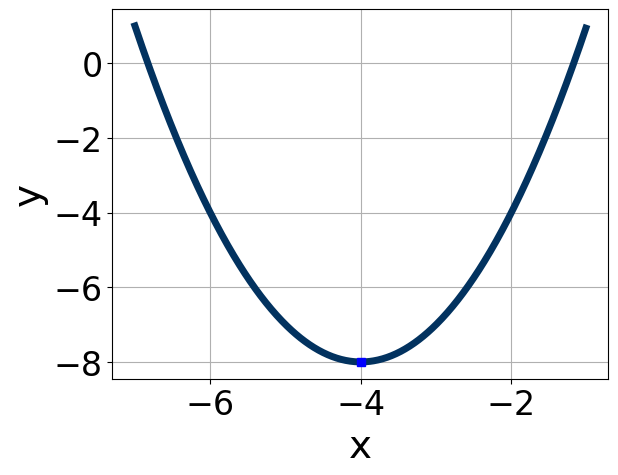
\includegraphics[width=0.5\textwidth]{../Figures/quadraticGraphToEquationC.png}
\end{center}
\begin{enumerate}[label=\Alph*.]
\item \( a \in [1, 2], \hspace*{5mm} b \in [8, 10], \text{ and } \hspace*{5mm} c \in [5, 9] \)
\item \( a \in [1, 2], \hspace*{5mm} b \in [-8, -7], \text{ and } \hspace*{5mm} c \in [23, 28] \)
\item \( a \in [1, 2], \hspace*{5mm} b \in [-8, -7], \text{ and } \hspace*{5mm} c \in [5, 9] \)
\item \( a \in [-4, 0], \hspace*{5mm} b \in [-8, -7], \text{ and } \hspace*{5mm} c \in [-24, -21] \)
\item \( a \in [-4, 0], \hspace*{5mm} b \in [8, 10], \text{ and } \hspace*{5mm} c \in [-24, -21] \)

\end{enumerate} }
\litem{
Solve the quadratic equation below. Then, choose the intervals that the solutions belong to, with $x_1 \leq x_2$ (if they exist).\[ -15x^{2} +7 x + 3 = 0 \]\begin{enumerate}[label=\Alph*.]
\item \( x_1 \in [-2.6, -0.5] \text{ and } x_2 \in [-0.72, 0.57] \)
\item \( x_1 \in [-0.6, 0.6] \text{ and } x_2 \in [0.57, 1.57] \)
\item \( x_1 \in [-11.3, -9.3] \text{ and } x_2 \in [3.88, 4.45] \)
\item \( x_1 \in [-16, -14.7] \text{ and } x_2 \in [15.11, 15.87] \)
\item \( \text{There are no Real solutions.} \)

\end{enumerate} }
\litem{
Factor the quadratic below. Then, choose the intervals that contain the constants in the form $(ax+b)(cx+d); b \leq d.$\[ 16x^{2} -32 x + 15 \]\begin{enumerate}[label=\Alph*.]
\item \( a \in [3.05, 4.89], \hspace*{5mm} b \in [-13, -3], \hspace*{5mm} c \in [3.94, 4.04], \text{ and } \hspace*{5mm} d \in [-6, 6] \)
\item \( a \in [0.13, 1.12], \hspace*{5mm} b \in [-23, -14], \hspace*{5mm} c \in [0.21, 1.02], \text{ and } \hspace*{5mm} d \in [-15, -9] \)
\item \( a \in [7.09, 8.31], \hspace*{5mm} b \in [-13, -3], \hspace*{5mm} c \in [1.11, 2.12], \text{ and } \hspace*{5mm} d \in [-6, 6] \)
\item \( a \in [1.86, 2.14], \hspace*{5mm} b \in [-13, -3], \hspace*{5mm} c \in [7.75, 8.12], \text{ and } \hspace*{5mm} d \in [-6, 6] \)
\item \( \text{None of the above.} \)

\end{enumerate} }
\litem{
Solve the quadratic equation below. Then, choose the intervals that the solutions belong to, with $x_1 \leq x_2$ (if they exist).\[ 20x^{2} +15 x -8 = 0 \]\begin{enumerate}[label=\Alph*.]
\item \( x_1 \in [-0.5, 1.1] \text{ and } x_2 \in [0.86, 2.17] \)
\item \( x_1 \in [-31.3, -29.6] \text{ and } x_2 \in [28.54, 30.04] \)
\item \( x_1 \in [-1.8, -0.4] \text{ and } x_2 \in [-0.03, 0.94] \)
\item \( x_1 \in [-23.4, -20.8] \text{ and } x_2 \in [6.73, 7.26] \)
\item \( \text{There are no Real solutions.} \)

\end{enumerate} }
\litem{
Solve the quadratic equation below. Then, choose the intervals that the solutions $x_1$ and $x_2$ belong to, with $x_1 \leq x_2$.\[ 15x^{2} -47 x + 36 = 0 \]\begin{enumerate}[label=\Alph*.]
\item \( x_1 \in [0.21, 0.55] \text{ and } x_2 \in [4.82, 5.52] \)
\item \( x_1 \in [19.99, 20.25] \text{ and } x_2 \in [26.53, 27.05] \)
\item \( x_1 \in [1.2, 1.5] \text{ and } x_2 \in [1.53, 2.31] \)
\item \( x_1 \in [0.5, 0.75] \text{ and } x_2 \in [3.81, 4.88] \)
\item \( x_1 \in [0.63, 0.97] \text{ and } x_2 \in [2.04, 2.96] \)

\end{enumerate} }
\litem{
Solve the quadratic equation below. Then, choose the intervals that the solutions $x_1$ and $x_2$ belong to, with $x_1 \leq x_2$.\[ 20x^{2} +69 x + 54 = 0 \]\begin{enumerate}[label=\Alph*.]
\item \( x_1 \in [-45.07, -44.94] \text{ and } x_2 \in [-24.02, -23.99] \)
\item \( x_1 \in [-2.34, -1.96] \text{ and } x_2 \in [-1.28, -1.13] \)
\item \( x_1 \in [-9.33, -8.66] \text{ and } x_2 \in [-0.37, -0.25] \)
\item \( x_1 \in [-7.1, -6.21] \text{ and } x_2 \in [-0.45, -0.33] \)
\item \( x_1 \in [-2.52, -2.38] \text{ and } x_2 \in [-1.18, -1.12] \)

\end{enumerate} }
\litem{
Graph the equation below.\[ f(x) = -(x-2)^2 + 11 \]\begin{enumerate}[label=\Alph*.]
\begin{multicols}{2}\item 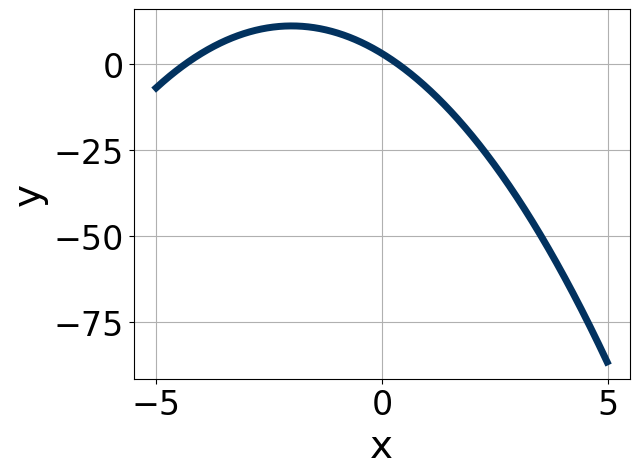
\includegraphics[width = 0.3\textwidth]{../Figures/quadraticEquationToGraphCopyAC.png}\item 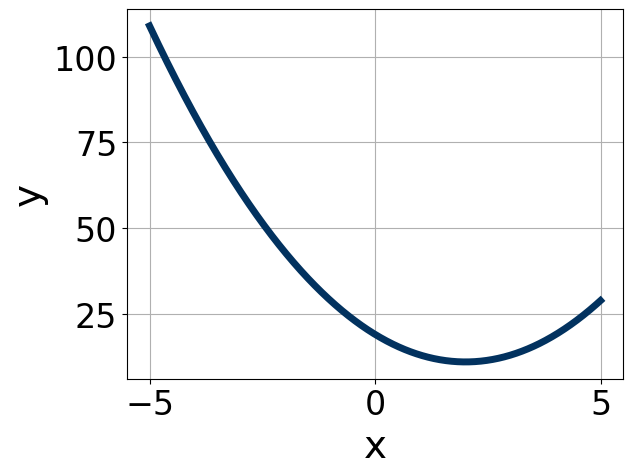
\includegraphics[width = 0.3\textwidth]{../Figures/quadraticEquationToGraphCopyBC.png}\item 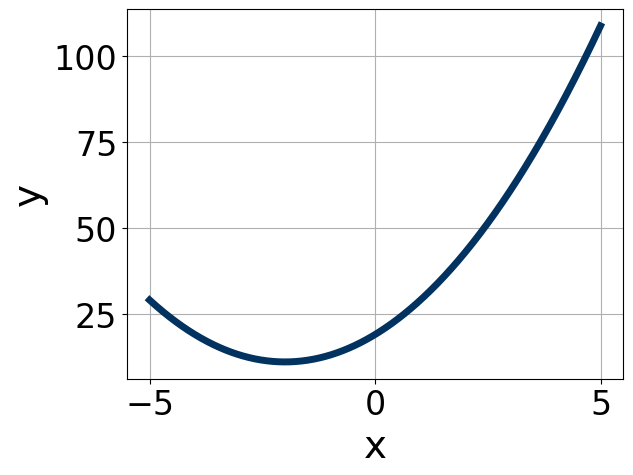
\includegraphics[width = 0.3\textwidth]{../Figures/quadraticEquationToGraphCopyCC.png}\item 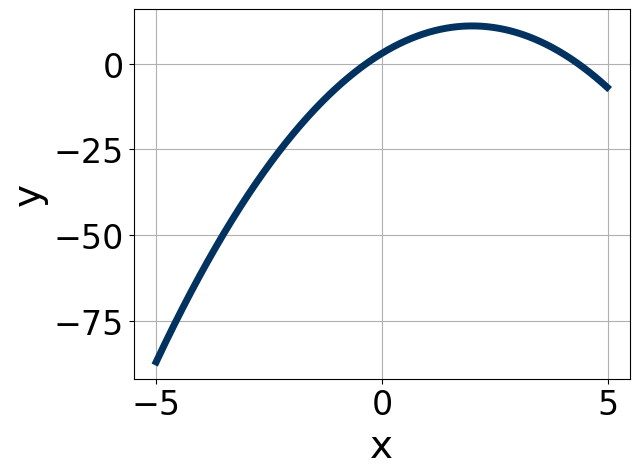
\includegraphics[width = 0.3\textwidth]{../Figures/quadraticEquationToGraphCopyDC.png}\end{multicols}\item None of the above.
\end{enumerate} }
\litem{
Factor the quadratic below. Then, choose the intervals that contain the constants in the form $(ax+b)(cx+d); b \leq d.$\[ 54x^{2} -33 x -10 \]\begin{enumerate}[label=\Alph*.]
\item \( a \in [3.3, 8], \hspace*{5mm} b \in [-7, 6], \hspace*{5mm} c \in [8.8, 10], \text{ and } \hspace*{5mm} d \in [-6, 4] \)
\item \( a \in [16.4, 20.8], \hspace*{5mm} b \in [-7, 6], \hspace*{5mm} c \in [1.5, 3.9], \text{ and } \hspace*{5mm} d \in [-6, 4] \)
\item \( a \in [1.3, 4.3], \hspace*{5mm} b \in [-7, 6], \hspace*{5mm} c \in [24.5, 27.9], \text{ and } \hspace*{5mm} d \in [-6, 4] \)
\item \( a \in [0.3, 1.3], \hspace*{5mm} b \in [-47, -44], \hspace*{5mm} c \in [-1.7, 2.3], \text{ and } \hspace*{5mm} d \in [8, 17] \)
\item \( \text{None of the above.} \)

\end{enumerate} }
\litem{
Write the equation of the graph presented below in the form $f(x)=ax^2+bx+c$, assuming  $a=1$ or $a=-1$. Then, choose the intervals that $a, b,$ and $c$ belong to.
\begin{center}
    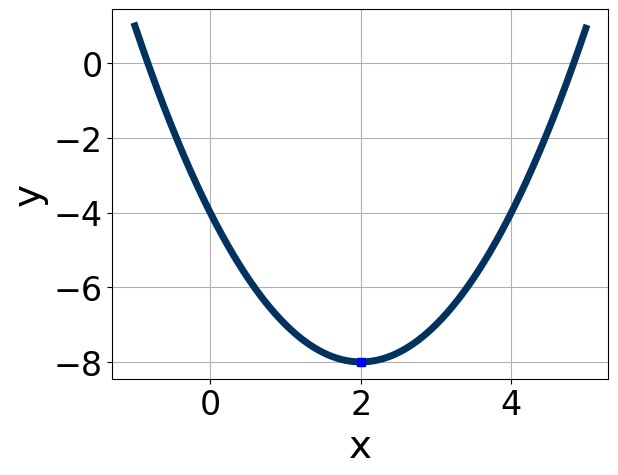
\includegraphics[width=0.5\textwidth]{../Figures/quadraticGraphToEquationCopyC.png}
\end{center}
\begin{enumerate}[label=\Alph*.]
\item \( a \in [1, 2], \hspace*{5mm} b \in [4, 5], \text{ and } \hspace*{5mm} c \in [-4, -1] \)
\item \( a \in [1, 2], \hspace*{5mm} b \in [4, 5], \text{ and } \hspace*{5mm} c \in [9, 14] \)
\item \( a \in [1, 2], \hspace*{5mm} b \in [-5, -1], \text{ and } \hspace*{5mm} c \in [-4, -1] \)
\item \( a \in [-2, 0], \hspace*{5mm} b \in [4, 5], \text{ and } \hspace*{5mm} c \in [-12, -9] \)
\item \( a \in [-2, 0], \hspace*{5mm} b \in [-5, -1], \text{ and } \hspace*{5mm} c \in [-12, -9] \)

\end{enumerate} }
\litem{
Graph the equation below.\[ f(x) = -(x+2)^2 - 20 \]\begin{enumerate}[label=\Alph*.]
\begin{multicols}{2}\item 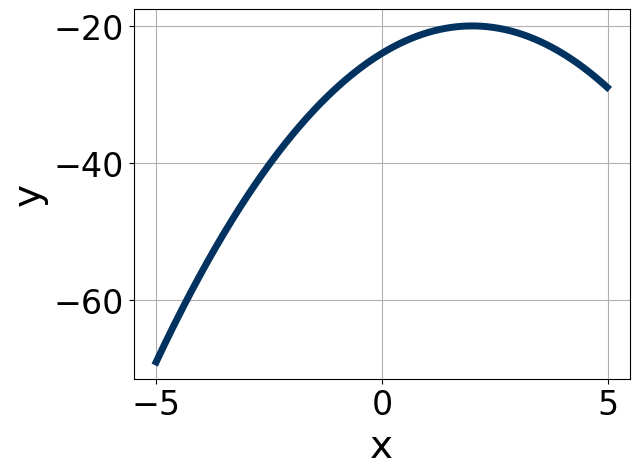
\includegraphics[width = 0.3\textwidth]{../Figures/quadraticEquationToGraphAC.png}\item 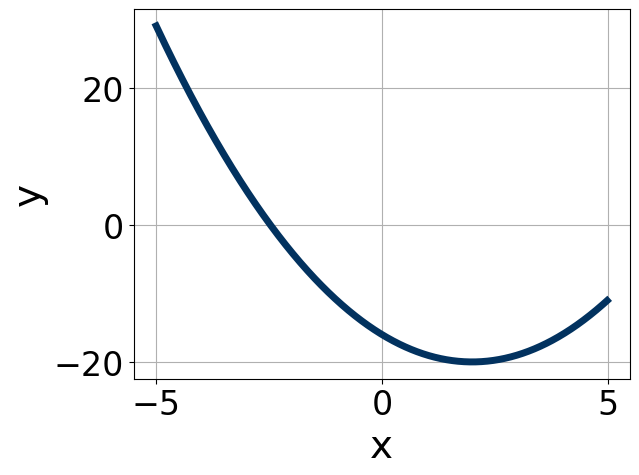
\includegraphics[width = 0.3\textwidth]{../Figures/quadraticEquationToGraphBC.png}\item 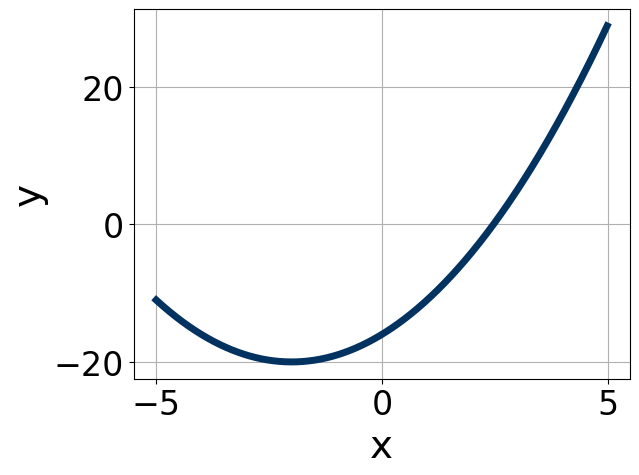
\includegraphics[width = 0.3\textwidth]{../Figures/quadraticEquationToGraphCC.png}\item 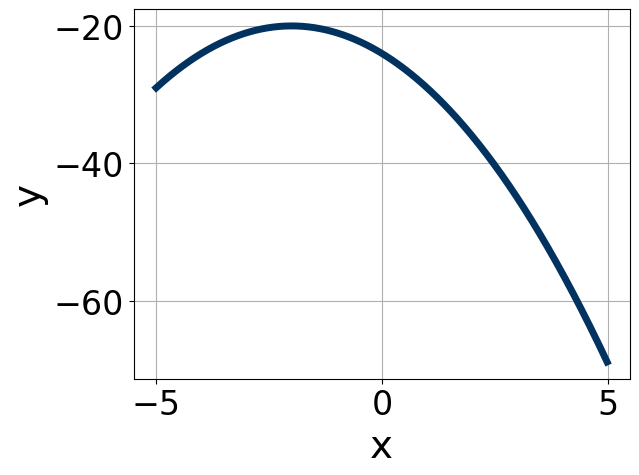
\includegraphics[width = 0.3\textwidth]{../Figures/quadraticEquationToGraphDC.png}\end{multicols}\item None of the above.
\end{enumerate} }
\end{enumerate}

\end{document}